\chapter{Testing \& Evaluation}

This chapter tests and evaluates the produced framework against the objectives and non-functional requirements outlined in \fullref{ch:objectives} using the environment outlined in \fullref{sec:testing_environment}.

\section{Recovering from a communication channel failure}
\label{sec:failure_recovery}

Communication failure can be caused by a variety of factors, but the most important to the covert system are caused by an adversary, especially in applications like censorship resistance.

I wrote a script to mimic an active warden (see \fullref{sec:filter_py} for implementation details), this script can block either one of the channels, or both. The script works by hooking into IPTables using a NetFilter queue, where it can drop and alter packets with the assistance of scapy \citep{scapy}. The script is rudimentary in its current state, as I do not have actual traffic to worry about disrupting, I can nullify header fields at my discretion. While the script sets the acknowledgement number to 0, in real-world application it would map these values in a fashion similar to that of Network Address Translation.

The clearest way to show this in action is to look at the script output during this process, to mimic this scenario I created the \url{FaucetEnv/Commblock} script, which calls the warden script (appendix \ref{sec:filter_py}).

\begin{figure}[H]
    \centering
    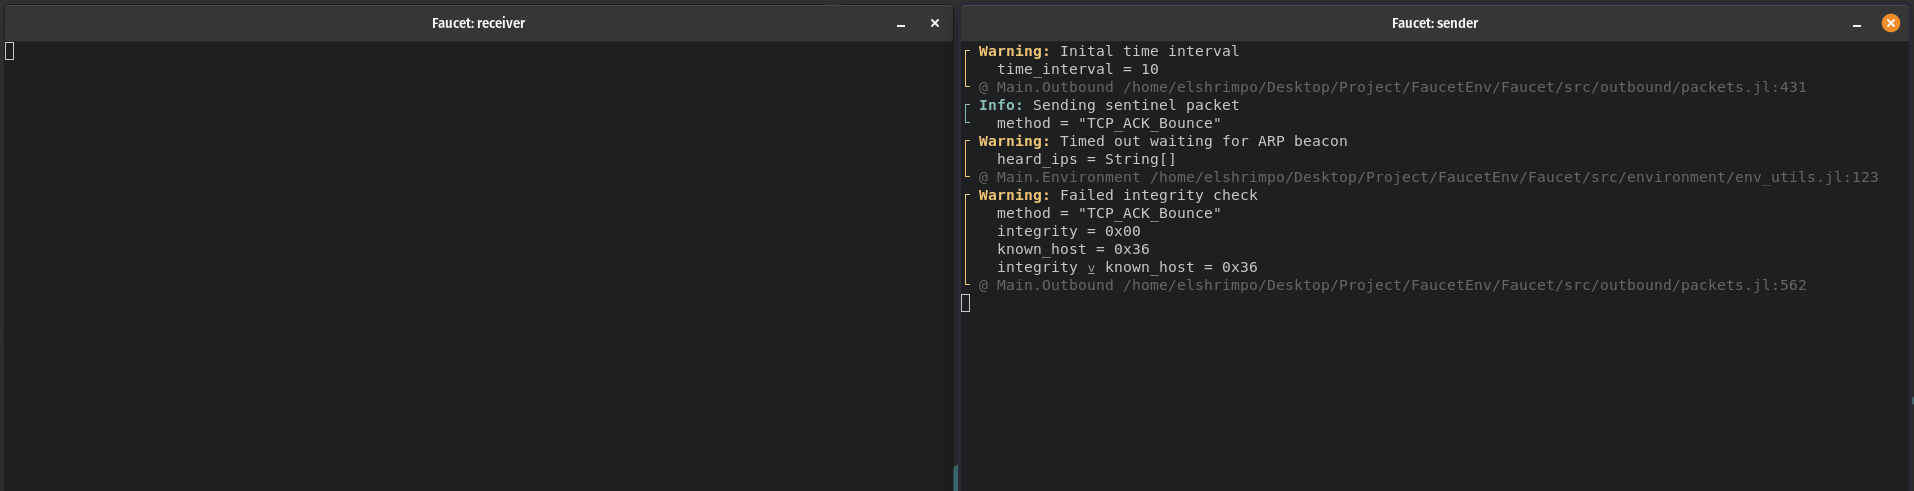
\includegraphics[width=\textwidth]{fig/TCP_Failure.png}
    \caption{TCP Channel failure}
    \label{fig:TCP_Failure}
\end{figure}

\begin{figure}[H]
    \centering
    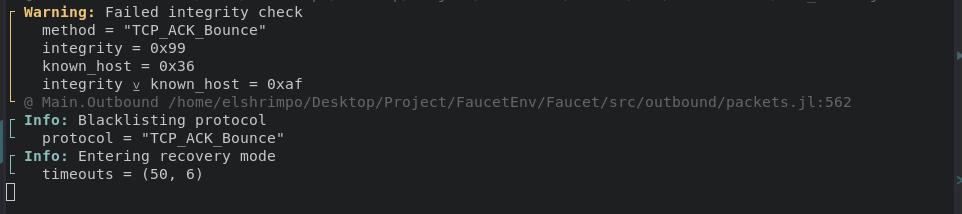
\includegraphics[width=0.9\textwidth]{fig/TCP_Fail_into_rec.png}
    \caption{TCP Channel fails again, starting the recovery process}
    \label{fig:TCP_Failure_again}
\end{figure}

\begin{figure}[H]
    \centering
    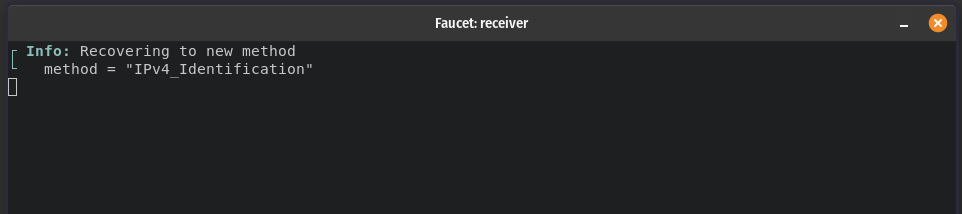
\includegraphics[width=0.9\textwidth]{fig/Recv_rec_resp.png}
    \caption{The receiver "recovers" to this new channel}
    \label{fig:recovery}
\end{figure}

\begin{figure}[H]
    \centering
    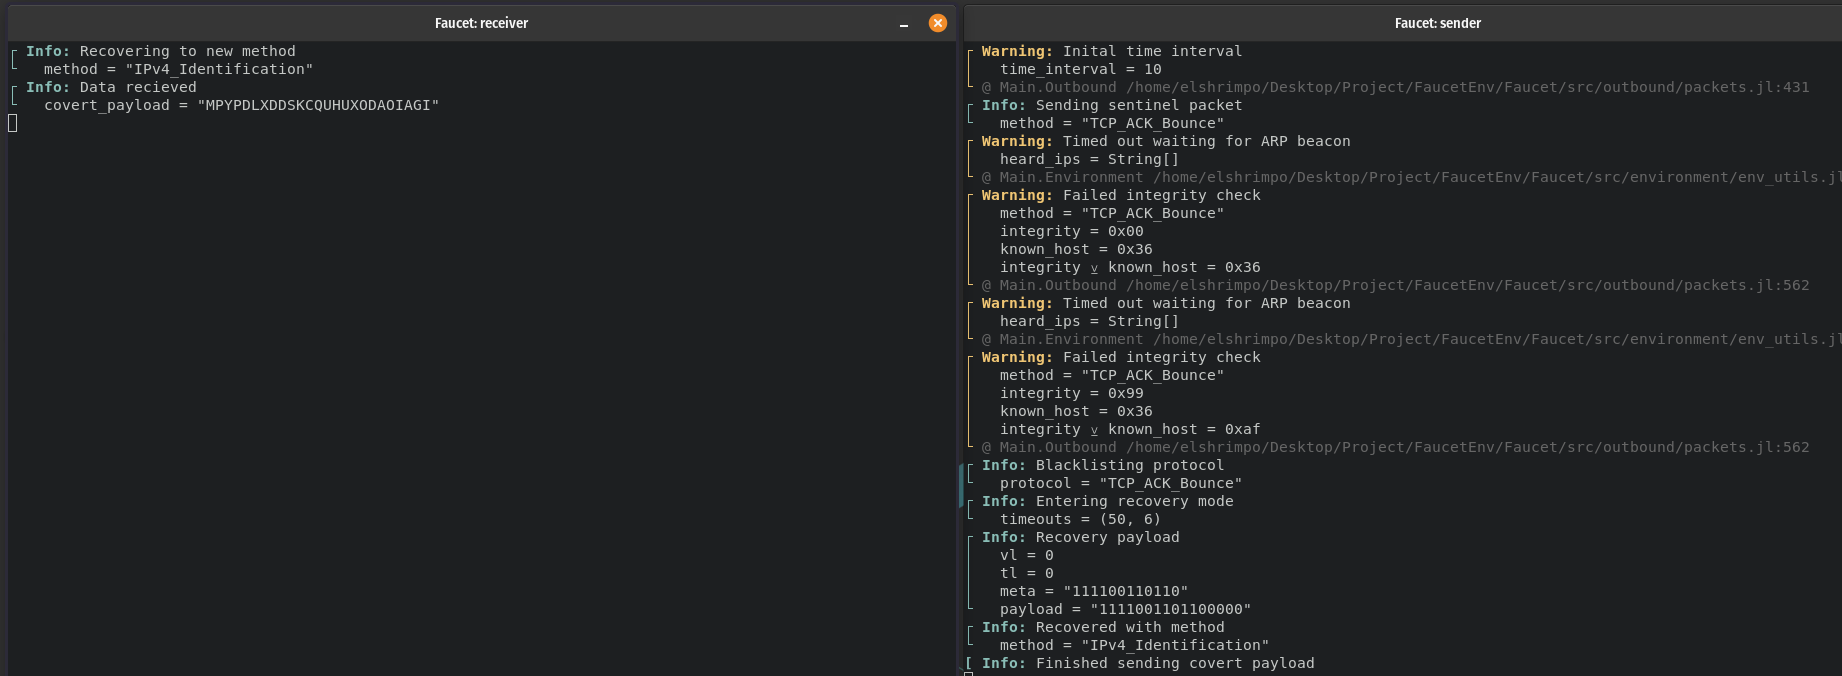
\includegraphics[width=\textwidth]{fig/Comm_works.png}
    \caption{Communication is restored, and successful}
    \label{fig:successful_comms}
\end{figure}

\begin{figure}[H]
    \centering
    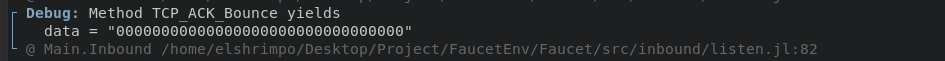
\includegraphics[width=0.9\textwidth]{fig/DEBUG_SHOW_WARDEN.png}
    \caption{The affect of the warden script on the packets}
    \label{fig:warden_affect}
\end{figure}

Running the testing script we can see that communication initially is unsuccessful (figure \ref{fig:TCP_Failure}), however, once the sender fails twice in a row with the same protocol, it blacklists the protocol and enters recovery mode (figure \ref{fig:TCP_Failure_again}). The sender waits before going into recovery mode to ensure the receiver is also in recovery mode. How these times are decided is outlined in \fullref{sec:channel_failures}. Once it sends the recovery packet to the receiver, the receiver will "recover" onto this new channel, that it knows is valid (figure \ref{fig:recovery}). Once the receiver has recovered, communication will continue as normal (although the original channel will remain blacklisted, and thus is unlikely to be used for a specified period). This can be seen in figure \ref{fig:successful_comms}.

By enabling the debug flag on the warden script, we can see how the warden affects the packets (figure \ref{fig:warden_affect}), where the acknowledgement field is set to 0.

This example shows that the framework can successfully recover from a communication channel failure, however, failures are not always as clear and simple as this, I doubt this approach is robust enough to handle all failures, but it does show it is possible. Managing the quality of channels is a complex task, but it would improve the availability of the system, especially when the environment is unreliable. This is an area that could be improved in future work.

\section{Transmission padding}
\label{sec:padding_testing}

The types of padding, outlined in \fullref{sec:transmission_padding}, are tested in this section.

The padding that works with a 1 followed by 0's for the remaining space will be referred to as "short" padding, and the padding proposed will be referred to as "covert" padding.

The drawback of covert padding over short padding is the additional space required to transmit the padding, however, due to the block size of AES encryption, the number of additional packets sent by this padding is negligible:

\begin{figure}[h]
    \centering
    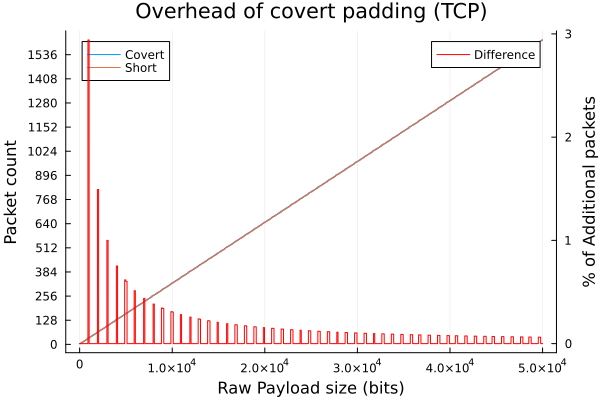
\includegraphics[width=0.7\textwidth]{fig/padding_size_TCP.png}
    \caption{The size of the padding required for a given payload size (TCP)}
    \label{fig:padding_size_TCP}
\end{figure}

\begin{figure}[h]
    \centering
    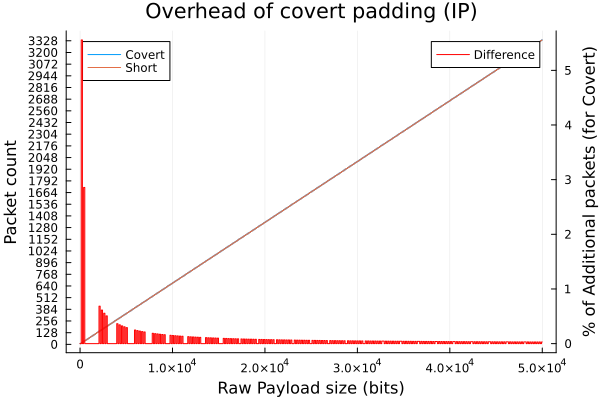
\includegraphics[width=0.7\textwidth]{fig/padding_size_IP.png}
    \caption{The size of the padding required for a given payload size (IP)}
    \label{fig:padding_size_IP}
\end{figure}

We can see here that the use of covert padding has very little effect on the number of packets sent, with the maximum being 5\% more packets sent for a payload (for IP). It is evident that the covert padding method is more effective for TCP, but for both protocols, they do not outperform the short padding method. By taking the number of payloads that require an extra packet to be sent, and dividing it by the total number of payloads, we get the percentage of packets that require an extra packet to be sent, multiplying that by the average percentage increase in packets sent, we can find the approximate overhead of the covert padding method:

Where $n$ is the number of payloads, $d$ is the number of $p$ that require an extra packet to be sent, $p_s$ is the average percentage increase in packets sent, and $o$ is the average overhead of the covert padding method, expressed as a percentage.

\begin{equation*}
    o = \frac{d}{n} * p_s * 100
\end{equation*}

The overhead for packets for TCP and IP is 1.02\% and 2.71\% respectively.

Where the covert padding method performs is in the distribution of the bits, where fields are supposed to be random, or unique, the percentage of 0's should be approximately 50\%, however, with short padding, this is not the case:

\begin{figure}[h]
    \centering
    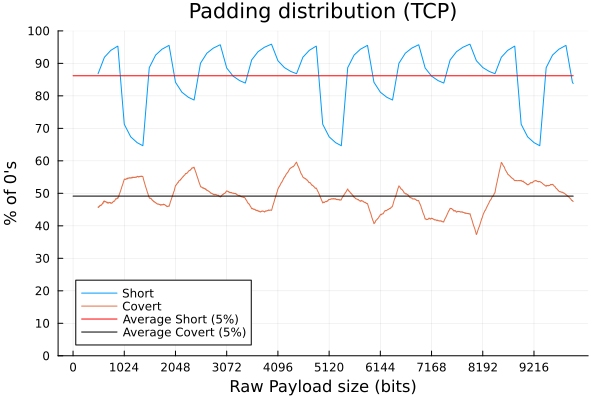
\includegraphics[width=0.7\textwidth]{fig/padding_distribution_TCP.png}
    \caption{A comparison of bit distributions in the TCP header with short padding and covert padding}
    \label{fig:padding_distribution_TCP}
\end{figure}

\begin{figure}[h]
    \centering
    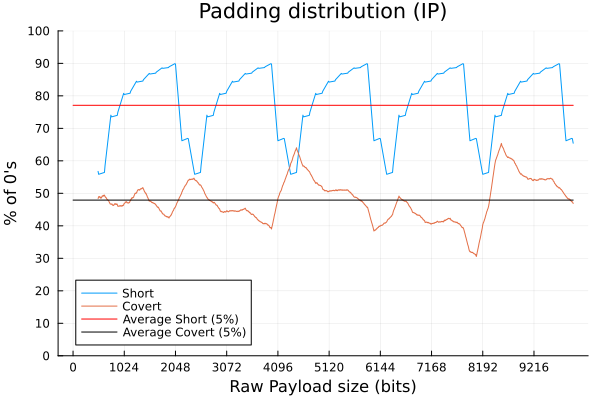
\includegraphics[width=0.7\textwidth]{fig/padding_distribution_IP.png}
    \caption{A comparison of bit distributions in the IP header with short padding and covert padding}
    \label{fig:padding_distribution_IP}
\end{figure}

We can see here that the covert padding method is much closer to the ideal distribution than the short padding method. We can also see that again, the larger field of the TCP header is better suited to the covert padding method, with a tighter distribution than the IP header. The covert headers are not perfect, because the size of the data always starts with a 0, which is required for the padding to be removed, however, this difference is negligible and would not be statistically significant.

\section{Testing the covertness of communication}

AES has passed the randomness test, and the padding method has a distribution that is much close to the ideal (with negligible variation), some other parts of communication can introduce patterns that reduce the covertness of the communication. These include the micro protocols and the random padding that follows them.

Extracting the IP Identification field from the captures of 256 communications, we can see that the distribution of the bits is not random and that there is a clear pattern to the data:

\begin{figure}[h]
    \centering
    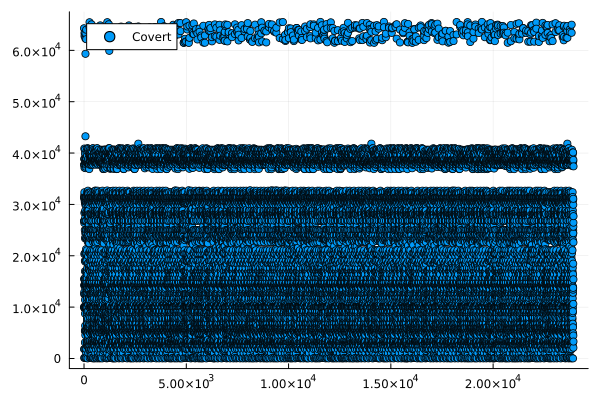
\includegraphics[width=0.7\textwidth]{fig/covert.png}
    \caption{The distribution of the bits in the IP Identification field}
    \label{fig:Covert_field}
\end{figure}

\begin{figure}[h]
    \centering
    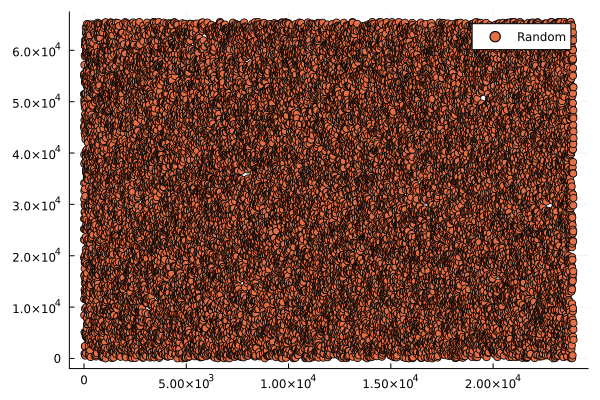
\includegraphics[width=0.7\textwidth]{fig/random.png}
    \caption{A Random distribution of a UInt16 field}
    \label{fig:RandomUInt16}
\end{figure}

\begin{figure}[h]
    \centering
    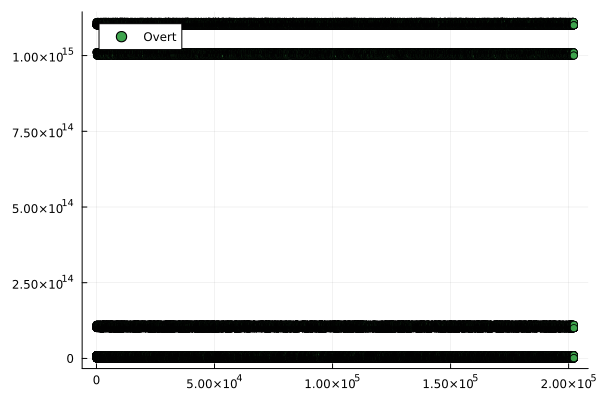
\includegraphics[width=0.7\textwidth]{fig/overt.png}
    \caption{The distribution of the bits in overt traffic fields}
    \label{fig:overt_field}
\end{figure}

I am unsure what exactly causes the distributions to look like this, but I suspect it is something related to micro protocols, the sparse nature of the points at the top of the graph is likely an artefact of the first bit that denotes data (0 for data, 1 for meta protocol), since our communication is more data than meta protocol, this is to be expected. However, neither of these distributions matches the overt data (figure \ref{fig:overt_field}), which is undesirable. This could open the framework up to detection methods that look for these patterns, however, as I am unaware of the cause of these patterns, I am unsure how to detect them.

\section{Testing channel selection and adaption}
\label{sec:channel_selection_and_adaption}

The framework can effectively select the best channel for the current situation. It will attempt to choose the channel with the highest bandwidth, while still factoring in covertness. Unfortunately showing this in a figure is difficult. The first channel is always chosen to do the sentinel, but it is not always the best suited, in a TCP-biased environment (like the one seen in figure \ref{fig:env_composition}) the IP Identification is not out of place, but it does have half capacity of the TCP Acknowledgement bounce, so it will immediately switch (see figures \ref{fig:send_switch} \& \ref{fig:recv_switch}).

\begin{figure}[h]
    \centering
    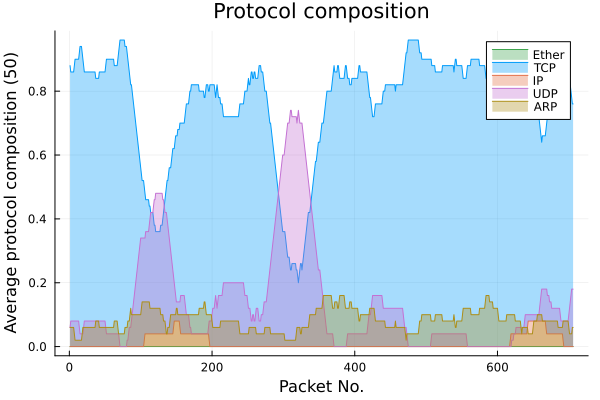
\includegraphics[width=0.7\textwidth]{fig/environment_composition.png}
    \caption{The composition of the environment}
    \label{fig:env_composition}
\end{figure}

\begin{figure}[h]
    \centering
    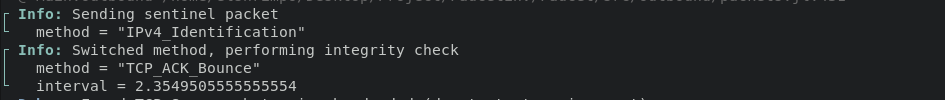
\includegraphics[width=0.7\textwidth]{fig/sender_adapt.png}
    \caption{Sender adapting to the environment}
    \label{fig:send_switch}
\end{figure}

\begin{figure}[h]
    \centering
    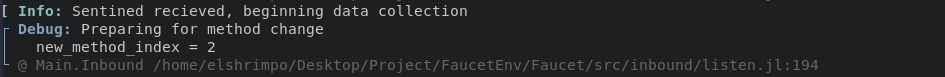
\includegraphics[width=0.7\textwidth]{fig/receiver_adapt.png}
    \caption{Receiver switching communication channel}
    \label{fig:recv_switch}
\end{figure}

\section{Testing detection and recovery from failures}
\label{sec:soft_failure_recovery}

The framework can detect failures in communication using the integrity challenge, under normal circumstances the integrity of the payload will not be compromised, however, by running the warden script (see \fullref{sec:filter_py}) we can compromise a section of communication, and see the framework recover from it.

\begin{figure}[h]
    \centering
    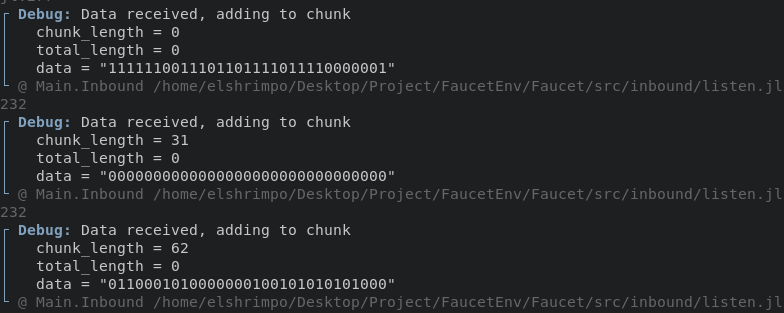
\includegraphics[width=0.7\textwidth]{fig/poison_tcp.png}
    \caption{A compromised payload}
    \label{fig:poison_tcp}
\end{figure}

\begin{figure}
    \centering
    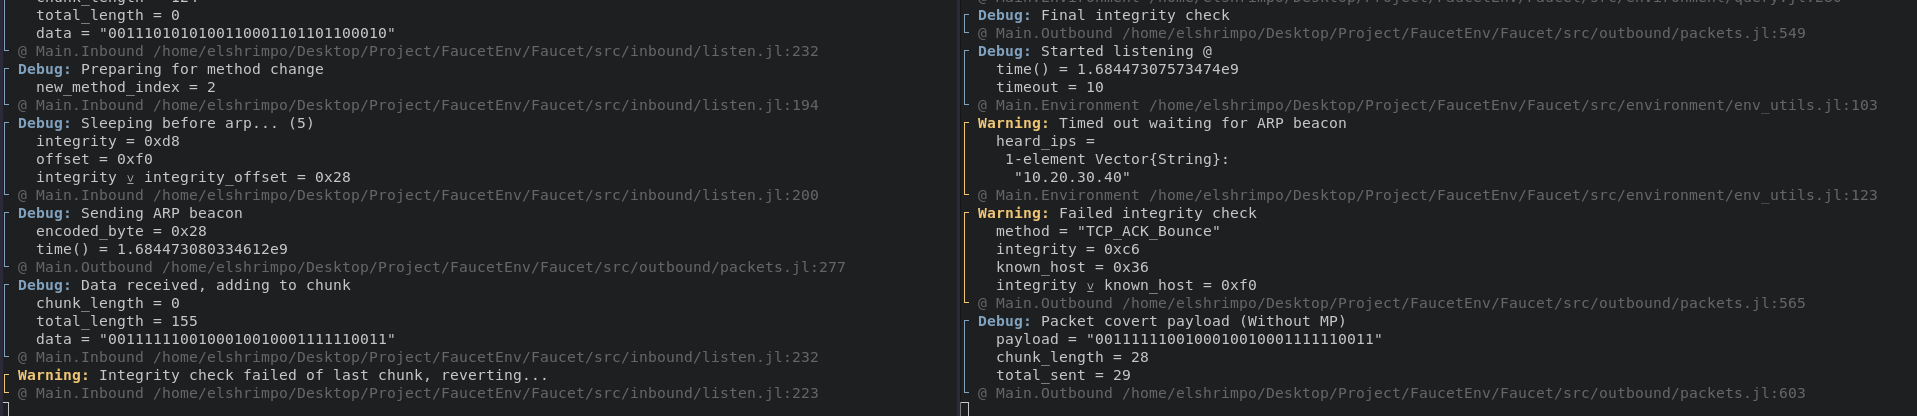
\includegraphics[width=0.7\textwidth]{fig/discard_posioned_chunk.png}
    \caption{The discarding of the compromised chunk}
    \label{fig:discard_poison}
\end{figure}


\begin{figure}
    \centering
    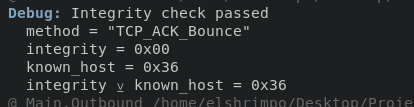
\includegraphics[width=0.7\textwidth]{fig/integrity_challenge.png}
    \caption{The sender sending an integrity challenge}
    \label{fig:integrity_challenge}
\end{figure}

\begin{figure}
    \centering
    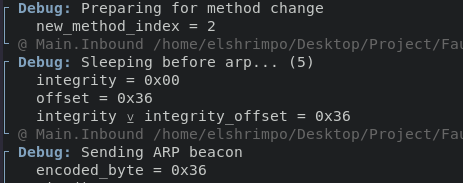
\includegraphics[width=0.7\textwidth]{fig/integrity_response.png}
    \caption{The receiver responding to the integrity challenge}
    \label{fig:integrity_response}
\end{figure}

Figure \ref{fig:poison_tcp} shows the compromised payload (the middle one), where the field has been altered, when the sender next sends an integrity challenge, the receiver will respond with the incorrect value, and the sender will inform it to discard the last chunk of data, see figure \ref{fig:discard_poison}. Conversely, if the receiver sends the correct value, the sender will continue as normal, see figures \ref{fig:integrity_challenge} \& \ref{fig:integrity_response}.

The framework successfully meets all of the \textit{\textbf{MUST}} requirements outlined:

\begin{itemize}
    \item The framework can determine the best communication channel for the current situation, as shown in \fullref{sec:channel_selection_and_adaption}.
    \item The framework can adapt to its environment, as shown in \fullref{sec:channel_selection_and_adaption}.
    \item The framework can detect and recover from failures in communication, as shown in \fullref{sec:soft_failure_recovery}.
    \item The framework uses encrypted communication, with a pre-shared key, as outlined in \fullref{sec:target}.
\end{itemize}

The framework also meets the \textit{\textbf{SHOULD}} requirement:

"The framework can recover from the complete failure of a communication channel", as shown in \fullref{sec:failure_recovery}.

However the requirement:

"Allow bidirectional communication" is not met, and I think is not possible for the framework to meet this requirement without large refactoring. While the framework does technically allow for bidirectional communication, this is simply limited to a response to a message, not a full conversation. For this system to be capable of bidirectional communication both parties would have to be able to agree on a channel that suits both of their environments, this would require more information to be shared between the parties and a more complex selection algorithm, additionally, this would impose a penalty on the response time of the system to a change in the environment.

The \textit{\textbf{MAY}} requirement:

"[The framework can] handle multiple channels at a time" is also not met. The additional complexity of this requirement is not worth the benefit, although if only direct channels (Ones that go straight from the sender to the receiver) are used, the receiver could reasonably handle multiple channels by tracking the source of the packets. However, this would prevent the use of some channels, such as the TCP Acknowledgement bounce that I utilise in this paper.

\section{Evaluation of non-functional requirements}

\subsection{The effect on covertness of the framework}

The use of multiple channels for communication allows for the framework to adapt to its environment, this is a great benefit to the covertness of the system, it also means that if a channel were to be discovered, for an adversary to extract the information they would have to work out the indexes of the relevant methods, which is a non-trivial task. 

The downside to using multiple channels for communication is that they require protocols, and protocols require a certain degree of structure. Where an adversary is aware of these protocols they could feasibly use them to detect the presence of a covert communication system. This is a problem that is not unique to this framework, but to all covert systems that use protocols.

The reduced covertness of the protocol structure is negligible in comparison to the benefits of multiple channels, as the search domain increases with the addition of more channels, and structure is easily mistaken for noise.

Writing a script to identify the channel is simple, however, identifying only the channel is much more difficult. It works by searching for the sentinel values in possible channels, in a clean environment (where the only traffic between the sender and receiver is the covert channel) this will detect the IP channel with 100\% accuracy, however, its false positive rate is much too high to say with certainty that a covert channel exists. This script is available in the appendix at \fullref{sec:warden_py}. The output of running this script on a pcap that only lasts for the duration of the covert channel can be seen in figure \ref{fig:warden_output}, where two of the identified sentinels are part of the covert channel.

\begin{figure}[H]
    \centering
    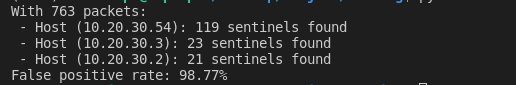
\includegraphics[width=0.7\textwidth]{fig/rudimentary_warden.png}
    \caption{The output of the rudimentary warden script}
    \label{fig:warden_output}
\end{figure}

This script does not represent the true covertness of the channel well, as it assumes the sender knows the channels in the communication. it also assumes the sentinel value, but there is no reason why the sentinel value could not be changed. For example, one's complement could be applied to all the encoded data, flipping all the bits, this would mean that the sentinel value would be 0000, which would evade this form of detection with no performance loss (but it would have to be agreed beforehand).

This type of warden also fails to properly detect the TCP Acknowledgement bounce channel, as the script sees the acknowledgement from the bouncing server, as opposed to the sender, which makes correctly identifying the start/end of a channel incredibly difficult.

For a more accurate warden, it would have to be aware of the following:

\begin{itemize}
    \item The covert methods that are being used.
    \item The sentinel value used.
    \item The index of each method (so it can "follow" the communication).
\end{itemize}

This is a difficult task, but perhaps could be done using a machine learning approach, where the warden is trained on a set of known channels, and then tested on an unknown channel. This would be a good area for future work.

To conclude this evaluation, it is easy to identify a possible covert channel, however, it is incredibly hard to identify the channel with certainty, even when the warden has knowledge of the implementation. Regardless of whether detection is possible retrospectively, it would require the channel to have already ended for communication to be identifiable. additionally, the solution for finding a channel is not of linear complexity, as the number of channels increases, the number of possible combinations increases exponentially. So the channel cannot be identified with certainty in real-time, or possibly at all, meaning it is incredibly covert.

\subsection{Application of the framework to real-world scenarios}

While the framework is proven to work inside a controlled environment, I doubt it would work in a real-world scenario. Given the complexity of the implementation, and my limited time, I have made shortcuts in the framework, the majority of my concern lies with the micro protocols, as I suspect they will be prone to interference from legitimate communication. While my channel can handle them being set to nothing, if they happened to be set to the right combination of values it could cause the channel to fail. There are also variable definitions, like the time to wait for a response to an integrity challenge, which has been arbitrarily set, and may not be suitable for all environments.

Another issue is the size of the framework, because of julias (current) lack of compilation, the entire standard library is required to run the framework, this is a large overhead and would be a problem in real-world applications where the sender is trying to remain undetected by the host it is running on. For scenarios where this is not an issue, like censorship resistance, this is not as much of an issue, although it does mean it requires more resources to run.


\subsection{Capability to add new communication channels}
\label{sec:new_channels}

Adding new channels to the framework is relatively simple, especially for channels that use already-supported protocols (such as IP or TCP), adding new protocols does however require additional work, as the receiver and sender will require a way to represent the protocol as a \inline{Packet} (see \fullref{sec:packet_processing}), and a way to create the packet from a dictionary (see \fullref{sec:sending_packets}) respectively.

While these tasks are not particularly arduous, for somebody unfamiliar with the language they may struggle to understand the codebase, and the lack of documentation regarding the addition of new channels may also be a hindrance.

This is an area that could be improved in future work, by adding documentation and examples or perhaps creating a tool that parses a protocol from a header file and generates the required code.

However, the only way to avoid this problem would be to use a language with support for these packets, such as C, however, this would not come without its problems. For example, C has support for these headers, but it is not as easy to understand or add to the codebase as Julia, conversely, Python is easy to understand and add to, but comes with performance limitations and a lack of portability (Note that Julia does not yet have a stable compilation process, but it is under development).

An implementation of a covert channel can be seen in \fullref{sec:impl_cov_mod}.